\documentclass{beamer}
\usepackage{lsfolien}
\usepackage[english]{babel}
\usepackage[utf8]{inputenc}

\myfootline{System Modelling and Semantic Web -- Spring 2021}{Hans-Gert Gräbe}

\title{Modelling Sustainable Systems\\ and Semantic Web\\[6pt]
  Modelling Contradictory Requirements in TRIZ
  \vskip1em}

\subtitle{Lecture in the Module 10-202-2309\\ for Master Computer Science}

\author{Prof. Dr. Hans-Gert Gräbe\\
\url{http://www.informatik.uni-leipzig.de/~graebe}}

\date{April 2021}
\begin{document}

{\setbeamertemplate{footline}{}
\begin{frame}
  \titlepage
\end{frame}}

\section{Basics}
\begin{frame}{Notion of a Technical System}

(V. Petrov, 2020) 

A \textbf{system} is a set of \emph{elements} which are \emph{interconnected}
and \emph{interact with each other}, which form a \emph{unified whole} which
has \emph{properties} that are not already contained in the constituing
elements considered individually.  

Such a property is referred to as a \textbf{system effect}, \textbf{synergy},
or \textbf{emergence}.

\textbf{Synergy} is the overall effect of the interaction of two or more
factors, characterised by the fact that this overall effect clearly exceeds
the effect of each of the components and their simple sum.
\end{frame}

\begin{frame}{TS as Reduction to the Essential}
  \begin{block}{The reduction to the essential ... }
    ... focuses on the following three dimensions:
    \begin{itemize}
    \item[(1)] Delimitation of the TS from the outside against an
      \emph{environment}, reduction of this relationships to input/output
      relations and guaranteed throughput (Purpose and ability to work).
    \item[(2)] Delimitation of the TS from the inside by grouping parts as
      \emph{components}, reducing their functioning on a "behavior control"
      via their interfaces.
    \item[(3)] Reduction of the relationships in the TS itself to
      \emph{causally essential} ones.
    \end{itemize}
  \end{block}
\end{frame}

\begin{frame}{Technical Systems and Antecedence}
  \begin{block}{The TS in the World of Technical Systems}
    The description of a TS is only possible based on descriptions of other
    (explicitly or implicitly given) TS. The description is anteceded ...
    \begin{itemize}
    \item[(1)] ... by a vague idea of the (working) input/output
      characteristics of the environment.
    \item [(2)] ... by a clear understanding how the components work beyond
      their pure specification.
    \item [(3)] ... by a vague idea of cause and effect relationships in the
      system itself, that precedes the detailed modeling.
    \end{itemize}
  \end{block}
\end{frame}

\begin{frame}{Components and Objects}
  (Szyperski 2002)
  \begin{itemize}
  \item Components are again systems.
  \item They can be self-developed or purchased from third parties. 
  \item It is not necessary to purchase the whole component, it is sufficient
    to use the \emph{service}.
  \end{itemize}
  This happens in many cases: A component is available in the system with its
  functional specification as a black box, the operation of the component
  (provision of the function) is carried out by a third party, out of
  \emph{their} area of responsibility,  the function has an effect on "my"
  objects in \emph{my area of responsibility}.
  \begin{itemize}
  \item Thus the distinction according to Szyperski: components encapsulate
    functionality, objects encapsulate system states. 
  \end{itemize}
\end{frame}

\begin{frame}{The Minimal Technical System in TRIZ}

\begin{center}
  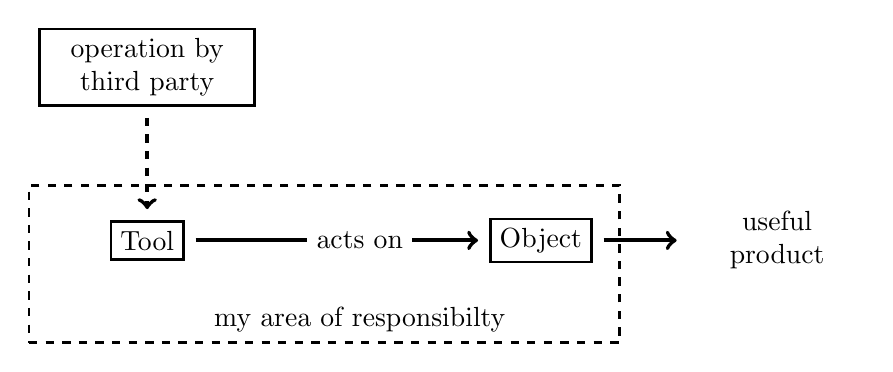
\begin{tikzpicture}[line width=1pt,
      pfeil/.style={shorten <=4pt, shorten >=4pt, line width=1.5pt},
      mytext/.style={text width=2.5cm,align=center}]
    \node[draw] at (0,1.3) [rectangle] (A0) {Tool};
    \node[draw] at (5,1.3) [rectangle] (A2) {Object};
    \node[text width=2cm,align=center] at (8,1.3) [rectangle] (A3) {useful
      product}; 
    \node[draw,mytext] at (0,3.5) [rectangle] (A4) {operation by third party};
    \draw[pfeil,->] (A0)--(A2) ;
    \draw[pfeil,->] (A2)--(A3) ;
    \draw[pfeil,->,dashed] (A4)--(A0) ;
    \draw[dashed] (-1.5,0) -- (6,0) -- (6,2) -- (-1.5,2) -- cycle ;
    \node[fill=white] at (2.7,1.3) [rectangle] {acts on};
    \node[] at (2.7,.3) {my area of responsibilty};
  \end{tikzpicture}
\end{center}
Dotted frame = the minimum technical system

Dotted arrow = is addressed in Szyperski, but not in TRIZ 
\end{frame}

\begin{frame}{Components and Environment}  
  Components (especially those operated by third parties) are thus pointers to
  other places in the \emph{world of technical systems} and thus represent
  only another form of the "relationship of a system to the environment".
  
  The question arises whether aspects (1) and (3) in the list of the
  "reductions to essential" (component and neighboring system) can be unified
  in such a way.  

  On the other hand, the question arises how to incorporate the concept of the
  object into the overall logic. 

  We will leave both questions open at this point. 
\end{frame}

\begin{frame}{Modelling of Systems}
  Two problems:
  \begin{itemize}
  \item[(1)] Build a new system
  \item[(2)] Transform an existing system
  \end{itemize}
  (1) can be considered as a special case of (2), since any need for a new
  system comes with at least \emph{rough ideas} about that new system, thus
  also under (1) there is at least a \emph{rough description form}
  of the system to be created as antecendence.
\end{frame}

\begin{frame}{Modelling of Systems}
\begin{center}
  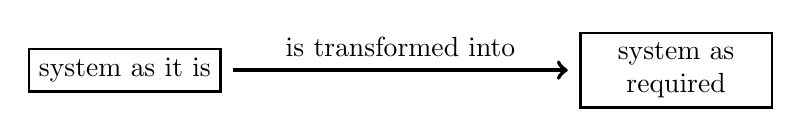
\begin{tikzpicture}[line width=1pt,
      pfeil/.style={shorten <=4pt, shorten >=4pt, line width=1.5pt},
      mytext/.style={text width=2.2cm,align=center}]
    \node[draw,mytext] at (0,0) [rectangle] (A0) {system as it is};
    \node[draw,mytext] at (7,0) [rectangle] (A2) {system as required};
    \draw[pfeil,->] (A0)--(A2) ;
    \node[fill=white] at (3.5,.3) [rectangle] {is transformed into};
  \end{tikzpicture}
\end{center}
  This basic scheme fits not only technical systems, but also the modelling of
  social, socio-ecological and cultural systems, hence it is sufficiently
  universal.
\end{frame}

\end{document}
